\documentclass[13pt]{beamer}
%
% Choose how your presentation looks.
%
% For more themes, color themes and font themes, see:
% http://deic.uab.es/~iblanes/beamer_gallery/index_by_theme.html
%
\mode<presentation>
{
\usetheme{CambridgeUS}     % or try Darmstadt, Madrid, Warsaw, ...
\usecolortheme{beaver} % or try albatross, beaver, crane, ...
\usefonttheme{default}  % or try serif, structurebold, ...
\setbeamertemplate{navigation symbols}{}
\setbeamertemplate{caption}[numbered]
} 

\usepackage[english]{babel}
\usepackage[utf8x]{inputenc}
\usepackage{xcolor}
\usepackage{multicol}
\usepackage{tikz}
\usepackage{tikz-uml}
\tikzumlset{font=\footnotesize\ttfamily}
\usepackage{hyperref}

\usepackage{listings}
\definecolor{codegreen}{rgb}{0,0.6,0}
\definecolor{codegray}{rgb}{0.5,0.5,0.5}
\definecolor{codepurple}{rgb}{0.58,0,0.82}
\definecolor{backcolour}{rgb}{0.95,0.95,0.92}

\lstdefinestyle{myCustomCppStyle}{
language=C++,
numbers=left,
stepnumber=1,
numbersep=9pt,
tabsize=2,
showspaces=false,
showstringspaces=false
}

\lstset{basicstyle=\tiny,style=myCustomCppStyle}

\lstdefinestyle{mystyle}{
backgroundcolor=\color{backcolour},   
commentstyle=\color{codegreen},
keywordstyle=\color{magenta},
numberstyle=\tiny\color{codegray},
stringstyle=\color{codepurple},
basicstyle=\ttfamily\footnotesize,
breakatwhitespace=false,         
breaklines=true,                 
captionpos=b,                    
keepspaces=true,                 
numbers=left,                    
numbersep=5pt,                  
showspaces=false,                
showstringspaces=false,
showtabs=false,                  
tabsize=1
}

\lstset{style=mystyle}

\usepackage{graphicx}
\graphicspath{ {./images/} }

\usepackage{tikz}
\usetikzlibrary{decorations.text}
\usetikzlibrary{shapes.geometric, arrows, positioning, calc, matrix}

\tikzset{
basic box/.style={
shape=rectangle, rounded corners, align=center,
draw=#1, fill=#1!25},
header node/.style={
Minimum Width=header nodes,
font=\strut\Large\ttfamily,
text depth=+0pt,
fill=white, draw},
header/.style={%
inner ysep=+1.5em,
append after command={
\pgfextra{\let\TikZlastnode\tikzlastnode}
node [header node] (header-\TikZlastnode) at (\TikZlastnode.north) {#1}
node [span=(\TikZlastnode)(header-\TikZlastnode)] at (fit bounding box) (h-\TikZlastnode) {}
}
},
hv/.style={to path={-|(\tikztotarget)\tikztonodes}},
vh/.style={to path={|-(\tikztotarget)\tikztonodes}},
fat blue line/.style={ultra thick, blue}
}

\definecolor{mygray}{RGB}{208,208,208}
\definecolor{mymagenta}{RGB}{226,0,116}
\newcommand*{\mytextstyle}{\sffamily\Large\bfseries\color{black!85}}
\newcommand{\arcarrow}[3]{%
% inner radius, middle radius, outer radius, start angle,
% end angle, tip protusion angle, options, text
\pgfmathsetmacro{\rin}{1.7}
\pgfmathsetmacro{\rmid}{2.2}
\pgfmathsetmacro{\rout}{2.7}
\pgfmathsetmacro{\astart}{#1}
\pgfmathsetmacro{\aend}{#2}
\pgfmathsetmacro{\atip}{5}
\fill[mygray, very thick] (\astart+\atip:\rin)
                 arc (\astart+\atip:\aend:\rin)
-- (\aend-\atip:\rmid)
-- (\aend:\rout)   arc (\aend:\astart+\atip:\rout)
-- (\astart:\rmid) -- cycle;
\path[
decoration = {
 text along path,
 text = {|\mytextstyle|#3},
 text align = {align = center},
 raise = -1.0ex
},
decorate
](\astart+\atip:\rmid) arc (\astart+\atip:\aend+\atip:\rmid);
}
\title[Design Pattern]{Behavioral Design Pattern}
\author{Hung Tran}
\institute{Fpt software}
\date{\today}


\begin{document}

\begin{frame}
\titlepage
\end{frame}

% Uncomment these lines for an automatically generated outline.
\begin{frame}{Outline}
\tableofcontents
\end{frame}

\section{Behavioral Pattern Overview}

\begin{frame}{Behavioral Pattern Overview}
	\begin{center}
	\textcolor{blue}{\textbf{Behavioral design patterns are concerned with algorithms and the assignment of responsibilities between objects.}}
	\end{center}
	\begin{itemize}
		\item \textbf{Chain of responsibility}: lets you pass requests along a chain of handlers.
		\item \textbf{Command}: turns a request into a stand-alone object that contains all information about the request.
		\item \textbf{Iterator}: lets you traverse elements of a collection without exposing its underlying representation (list, stack, tree, etc.).
		\item \textbf{Mediator}: lets you reduce chaotic dependencies between objects.
		\item \textbf{Memento}: lets you save and restore the previous state of an object without revealing the details of its implementation.
	\end{itemize}
\end{frame}

\begin{frame}{Behavioral Pattern Overview}
	\begin{itemize}
		\item \textbf{Observer}: lets you define a subscription mechanism to notify multiple objects about any events that happen to the object they’re observing.
		\item \textbf{State}: lets an object alter its behavior when its internal state changes. It appears as if the object changed its class.
		\item \textbf{Strategy}: lets you define a family of algorithms, put each of them into a separate class, and make their objects interchangeable.
		\item \textbf{Template Method}: defines the skeleton of an algorithm in the superclass but lets subclasses override specific steps of the algorithm without changing its structure.
		\item \textbf{Visitor}: lets you separate algorithms from the objects on which they operate.
	\end{itemize}
\end{frame}

\section{Iterator pattern}

\begin{frame}{Problem Statement: Collections}
	\begin{columns}[T]
		\begin{column}{.5\textwidth}
			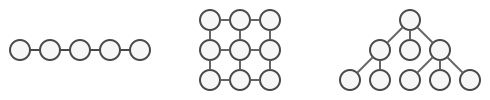
\includegraphics[scale=0.4]{./images/problem.png}
			\begin{itemize}
				\item Collections are based on stacks, trees, graphs and other complex data structures.
				\item But no matter how a collection is structured, it must provide some way of accessing its elements so that other code can use these elements. 
			\end{itemize}
		\end{column}
	
		\begin{column}{.5\textwidth}
			\begin{itemize}
				\item If you have a collection based on a list, you just loop over all of the elements.
				\item How do you sequentially traverse elements of a complex data structure, such as a tree?
				\item Depth-first traversal or breadth-first traversal.
			\end{itemize}
			\textcolor{red}{Clients not care how they store their elements?}
		\end{column}
	\end{columns}
\end{frame}

\begin{frame}{Solution: Iterator Design Pattern}
	\begin{columns}[T]
		\begin{column}{.5\textwidth}
			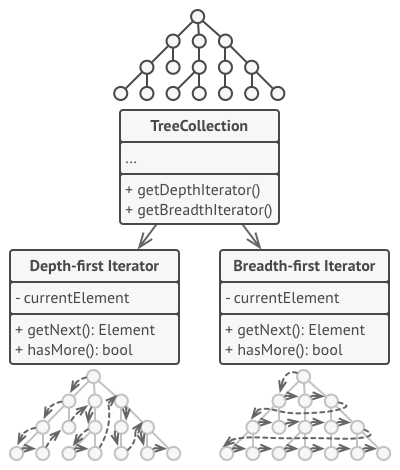
\includegraphics[scale=0.35]{./images/solution.png}
		\end{column}
	
		\begin{column}{.5\textwidth}
			\begin{itemize}
				\item An iterator object encapsulates all of the traversal details, such as the current position and how many elements are left till the end.
				\item Several iterators can go through the same collection at the same time, independently of each other.
				\item All iterators must implement the same interface. 
			\end{itemize}
		\end{column}
	\end{columns}
\end{frame}

\begin{frame}{The Intent of Iterator Design Pattern}
	\begin{center}
	\textcolor{red}{\textbf{Command is a behavioral design pattern that turns a request into a stand-alone object that contains all information about the request. This transformation lets you pass requests as a method arguments, delay or queue a request’s execution, and support undoable operations.}}\\
	\end{center}
\end{frame}

\begin{frame}{Structure of Iterator Pattern}
	\begin{center}
	\begin{tikzpicture}
 	\umlemptyclass[x=4,y=0]{Client}
 	\umlclass[x=0,y=0]{Aggregate}{}{createIter()}
 	\umlclass[x=8,y=0]{Iterator}{}{+first() \\ +next() \\ +isDone() \\ +currentItem()}
 	\umlclass[x=0,y=-4]{ConcreteAggregate}{}{+handlerRequest()}
 	\umlclass[x=8,y=-4]{ConcreteIterator}{}{+handlerRequest()}
 	\umluniassoc[pos=0.95, align=right, name=uniassoc]{Client}{Aggregate}
 	\umluniassoc[pos=0.95, align=right, name=uniassoc]{Client}{Iterator}
 	\umlinherit[geometry=|-|, pos=0.95, align=right, name=uniassoc]{ConcreteAggregate}{Aggregate}
 	\umlinherit[geometry=|-|, pos=0.95, align=right, name=uniassoc]{ConcreteIterator}{Iterator}
 	\umluniassoc[pos=0.95, align=right, name=uniassoc]{ConcreteIterator}{ConcreteAggregate}
	\end{tikzpicture}	
	\end{center}
\end{frame}

\begin{frame}{Applicability}
	\begin{itemize}
		\item Use the Iterator pattern when your collection has a complex data structure under the hood, but you want to hide its complexity from clients (either for convenience or security reasons).
		\item Use the pattern to reduce duplication of the traversal code across your app.
		\item Use the Iterator when you want your code to be able to traverse different data structures or when types of these structures are unknown beforehand.
	\end{itemize}
\end{frame}

\begin{frame}{How to Implement}
	\begin{itemize}
		\item Declare the iterator interface. At the very least, it must have a method for fetching the next element from a collection. But for the sake of convenience you can add a couple of other methods, such as fetching the previous element, tracking the current position, and checking the end of the iteration.
		\item Declare the collection interface and describe a method for fetching iterators.
		\item Implement concrete iterator classes for the collections that you want to be traversable with iterators.
		\item Implement the collection interface in your collection classes. 
		\item Go over the client code to replace all of the collection traversal code with the use of iterators.
	\end{itemize}
\end{frame}

\begin{frame}{Pros and Cons}
	\begin{columns}[T]
		\begin{column}{.5\textwidth}
			\begin{itemize}
				\item Single Responsibility Principle. You can clean up the client code and the collections by extracting bulky traversal algorithms into separate classes.
				\item Open/Closed Principle. You can implement new types of collections and iterators and pass them to existing code without breaking anything.
				\item  You can iterate over the same collection in parallel because each iterator object contains its own iteration state.
				\item For the same reason, you can delay an iteration and continue it when needed.
			\end{itemize}
		\end{column}
	
		\begin{column}{.5\textwidth}
			\begin{itemize}
				\item Applying the pattern can be an overkill if your app only works with simple collections.
				\item Using an iterator may be less efficient than going through elements of some specialized collections directly.
			\end{itemize}
		\end{column}
	\end{columns}
\end{frame}

\begin{frame}{Relations with Other Patterns}
	\begin{itemize}
		\item You can use Iterators to traverse Composite trees.
		\item You can use Factory Method along with Iterator to let collection subclasses return different types of iterators that are compatible with the collections.
		\item You can use Memento along with Iterator to capture the current iteration state and roll it back if necessary.
		\item You can use Visitor along with Iterator to traverse a complex data structure and execute some operation over its elements, even if they all have different classes.
	\end{itemize}
\end{frame}

\begin{frame}
\begin{center}
{\fontsize{40}{50}\selectfont Thank You!}
\end{center}
\end{frame}

\end{document}
